\chapter{Conception du Datawarehouse}

\section*{Introduction}%
\addcontentsline{toc}{section}{\numberline{}Introduction}%
Ce chapitre est dédié à la conception de l’entrepôt de données de notre système de business intelligence. Nous allons commencer par présenter entièrement l’architecture du système à concevoir, puis nous allons concevoir chacune des parties qui constituent la mise en place d’un entrepôt de données. On débutera par le datawarehouse, duquel découlera les datamarts. Ensuite on passera à la conception des ETL qui seront chargés d’alimenter notre datawarehouse.

\section{Architecture du système de Business Intelligence}
Dans la phase d’analyse nous avons opté pour une plateforme de business intelligence. Ceci implique la conception du système des le début avec l’intégration des données jusqu’à la visualisation. 
\paragraph{}
Sur le plan technique et purement technique, la Business intelligence peut être caractérisée comme une famille d'outils progiciels bien spécifiques, chacun étant destiné à traiter une phase du processus décisionnel depuis la collecte de données au sein même des unités de production jusqu'à la facilitation de l'aide à la décision pour les managers. Voyons les caractéristiques typiques d'une plate-forme informatique décisionnelle, l'architecture du principe est ici classiquement présentée selon 4 étages.
\paragraph{}
La Business Intelligence (informatique décisionnelle) propose d'utiliser les données transitant par le Système d'information, données de production le plus souvent, en informations susceptibles d'être exploitées à des fins décisionnelles.

\begin{figure}[H]
    \centering
    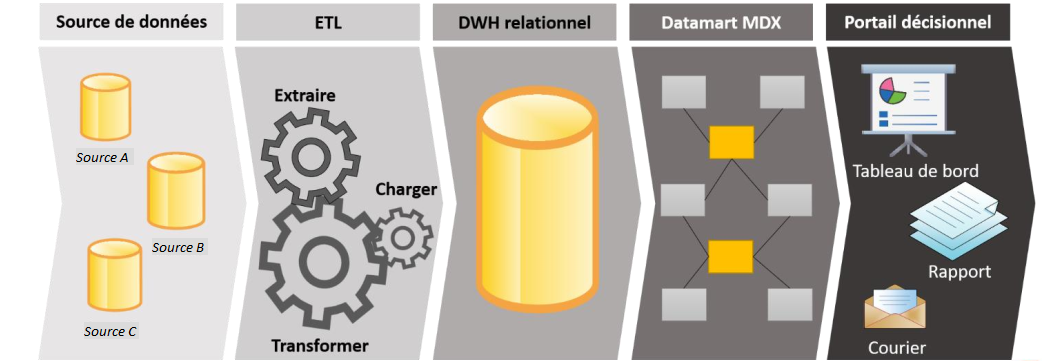
\includegraphics[width=\textwidth]{architecturesysteme}
    \caption{Architecture de notre Solution de Business Intelligence}
    \label{fig:architecturesysteme}
\end{figure}

La figure \ref{fig:architecturesysteme} montre l’architecture globale de notre système de business intelligence. On peut voir les 4 étages comme la transition entre les différents parties dans l'architecture.

\begin{itemize}
    \item \textbf{Collecter, nettoyer et consolider les données :} Extraire les données des systèmes de production et les adapter à un usage décisionnel. L'étage entre les sources de données et les processus ETL.
    \item \textbf{Stocker :} Centraliser les données structurées et traitées afin qu'elles soient disponibles pour un usage décisionnel. L'étage entre les processus ETL et le datawarehouse.
    \item \textbf{Distribuer :} Ou plutôt faciliter l'accessibilité des informations selon les fonctions et les types d'utilisation. L'étage entre le datawarehouse et les datamarts pour l'analyse.
    \item \textbf{Exploiter :} Ou comment assister du mieux possible l'utilisateur afin qu'il puisse extraire la substance de l'information des données stockées à cet usage. L'étage entre les datamarts et le portail décisionnel (les tableaux de bords).
\end{itemize}

\section{Conception du Datawarehouse et des Datamarts}
Les datawarehouse sont destinés à la mise en place de systèmes décisionnels. Ces systèmes, devant répondre à des objectifs différents des systèmes transactionnels, ont fait ressortir très vite la nécessité de recourir à un modèle de données simplifié et aisément compréhensible. La modélisation dimensionnelle permet cela. Elle consiste à considérer un sujet d’analyse comme un cube à plusieurs dimensions, offrant des vues en tranches ou des analyses selon différents axes.
\paragraph{}
La modélisation des bases de données relationnelles utilise les concepts d’entités et de relations afin de construire des tables. En business intelligence, la modélisation d’un datawarehouse (entrepôt de données) utilise les notions de table de faits et table de dimension. La figure \ref{fig:bddetdwh} extrait de la publication de Rachid SAAD\footnote{https://www.saadrachid.net/bi-big-data/modelisation-dun-datawarehouse/} sur la \textit{"MODÉLISATION D’UN DATAWAREHOUSE"} montre les différences entre la modélisation des bases de données et la modélisation d’un datawarehouse.

\begin{figure}[H]
    \centering
    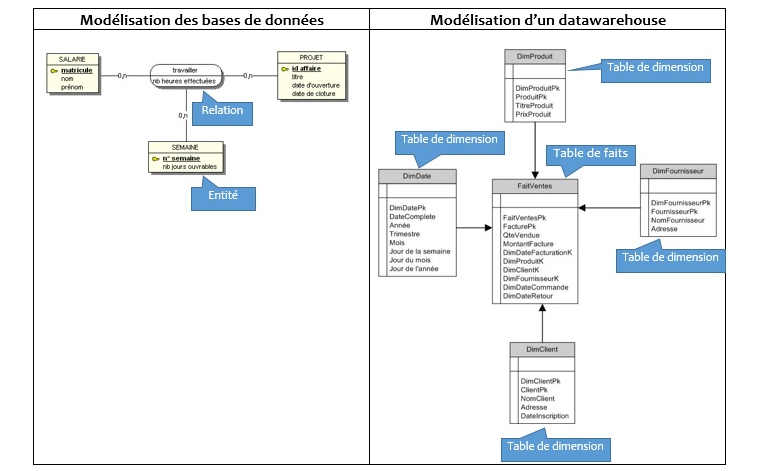
\includegraphics[width=\textwidth]{bddetdwh}
    \caption{Architecture basique de notre datawarehouse}
    \label{fig:bddetdwh}
\end{figure}

Mais d'abord parlons de l'architecture qu'aura le datawarehouse que nous voulons construire.

\subsection{Architecture du Datawarehouse}
Dans une architecture traditionnelle, il existe trois modèles communs de Data Warehouses : Data Warehouse virtuel, Data Mart et Data Warehouse d’entreprise :
\begin{itemize}
    \item \textbf{Un Data Warehouse virtuel :} C'est un ensemble de bases de données séparées, qui peuvent être interrogées ensemble, de sorte qu’un utilisateur peut accéder efficacement à toutes les données comme si elles étaient stockées dans un seul entrepôt de données.
    \item \textbf{Un modèle de Data Mart :}  C'est utilisé pour les rapports et les analyses spécifiques à un secteur d’activité. Dans ce modèle d’entrepôt de données, les données sont agrégées à partir d’une gamme de systèmes sources pertinents pour un domaine d’activité spécifique, comme les ventes ou la finance.
    \item \textbf{Un Data Warehouse d’entreprise :} Ceci implique que l’entrepôt de données doit contenir des données agrégées couvrant l’ensemble de l’organisation. Ce modèle considère l’entrepôt de données comme le cœur du système d’information de l’entreprise, avec des données intégrées provenant de toutes les unités d’affaires.
\end{itemize}

La structure du Data Warehouse d’une organisation dépend de sa situation actuelle et de ses besoins. La structure de base permet aux utilisateurs finaux de l’entrepôt d’accéder directement aux données sommaires dérivées des systèmes sources et d’effectuer l’analyse, la production de rapports et l’exploration de ces données. 

Nous allons implémenter un datawarehouse d'entreprise puisqu'elle répond le mieux a nos objectifs. La figure \ref{fig:architecturedwh} extrait du blog de Cartelis\footnote{https://www.cartelis.com/blog/architecture-data-warehouse}, représente bien l'architecture de notre datawarehouse.
\begin{figure}[H]
    \centering
    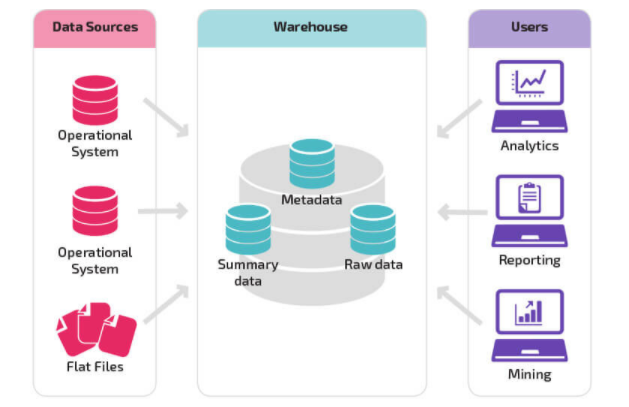
\includegraphics[width=\textwidth]{architecturedwh}
    \caption{Architecture basique de notre datawarehouse}
    \label{fig:architecturedwh}
\end{figure}

Cependent une zone staging est souvent nécessaire dans l'implémentation d'un datawarehouse. Comme mentionné plus haut, c'est la zone de préparation du datawarehouse. Dans la zone de préparation « Staging area » les données sont extraites à partir des sources de données, transformées et préparées pour le chargement final. Au niveau du serveur « ETL » il est procédé à l’affectation de clés artificielles et à quelques transformations nécessaires avant le chargement final dans la zone d’entreposage. Notre datawarehouse final aura une architecture comme dans la figure \ref{fig:architecturedwhfinal} extrait du même blog.

\begin{figure}[H]
    \centering
    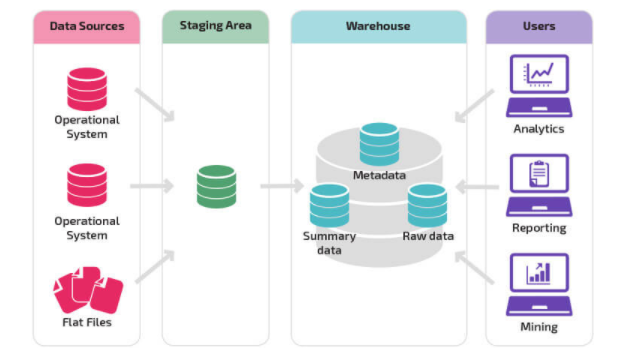
\includegraphics[width=\textwidth]{architecturedwhfinal}
    \caption{Architecture final de notre datawarehouse}
    \label{fig:architecturedwhfinal}
\end{figure}

\subsection{Modélisation dimensionnelle}
Dans un Data Warehouse (et au niveau de chaque Data mart), les données et leurs relations sont organisées suivant un modèle de données spécifique. Le diagramme \ref{fig:modeledimensionnel} qui représente un modèle dimensionnel ressemble à une étoile, avec une grande table centrale et un jeu de petites tables auxiliaires disposées en étoile autour de la table centrale. Celle-ci est appelée \textbf{table de faits} et les autres tables sont appelées \textbf{tables de dimensions}.

\begin{figure}[H]
    \centering
    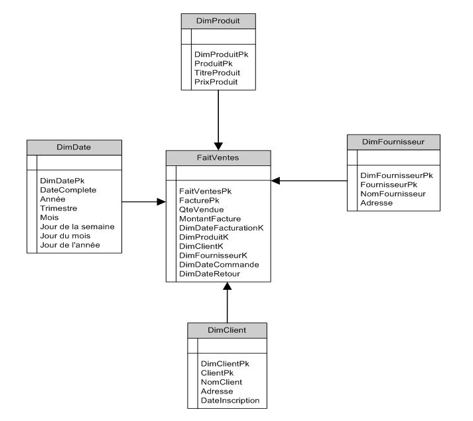
\includegraphics[width=\textwidth]{modeledimensionnel}
    \caption{Exemple de modèle dimensionnel de données}
    \label{fig:modeledimensionnel}
\end{figure}

\subsubsection{Qu’est-ce qu’une table de fait?}
Une table de faits est la table centrale du modèle dimensionnel. Elle contient les informations observables (les mesures) sur ce qu’on veut analyser : Table de faits des ventes par exemple. Une ligne d’une table de faits correspond à une mesure. Ces mesures sont généralement des valeurs numériques, additives ; cependant des mesures textuelles peuvent exister mais sont rares. Une table de faits assure les liens plusieurs à plusieurs entre les dimensions. Elles comportent des clés étrangères, qui ne sont autres que les clés primaires des tables de dimension. Un peu comme dans les figures \ref{fig:structuretabledesfaits} et \ref{fig:exempletabledesfaits}

\begin{figure}[H]
    \centering
    \begin{minipage}{.6\textwidth}
      \centering
      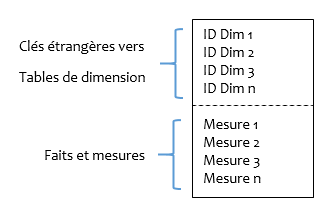
\includegraphics[width=.8\linewidth]{structuretabledesfaits}
      \captionof{figure}{Structure d'une table de faits}
      \label{fig:structuretabledesfaits}
    \end{minipage}%
    \begin{minipage}{.4\textwidth}
      \centering
      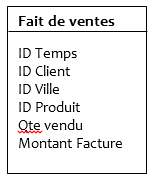
\includegraphics[width=.7\linewidth]{exempletabledesfaits}
      \captionof{figure}{Exemple d'une table de faits}
      \label{fig:exempletabledesfaits}
    \end{minipage}
\end{figure}

\subsubsection{Qu’est-ce qu’une table de dimension?}
Une table de dimension représente un axe d’analyse : dimension de temps, dimension géographique, dimension client, etc. Les tables de dimension sont les tables qui raccompagnent une table de faits, elles contiennent les descriptions textuelles de l’activité. Une table de dimension est constituée de nombreuses colonnes qui décrivent une ligne. C’est grâce à cette table que l’entrepôt de données est compréhensible et utilisable ; elles permettent des analyses en tranches et en dés. Une dimension est généralement constituée : d’une clé artificielle, une clé naturelle et des attributs. La figure \ref{fig:exempletablesdedimensions} illustre un exemple.

\begin{figure}[H]
    \centering
    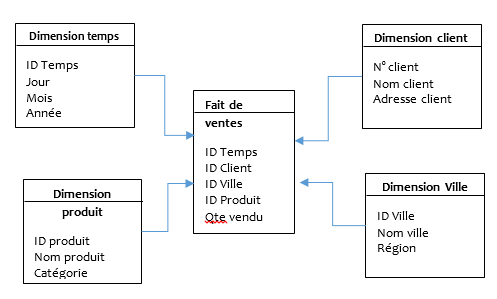
\includegraphics[width=\textwidth]{exempletablesdedimensions}
    \caption{Exemple de tables de dimension}
    \label{fig:exempletablesdedimensions}
\end{figure}

\subsection{Choix du modèle de schéma}
Trois modèles permettent la présentation d’un datawarehouse :
\begin{itemize}
    \item Modèle en étoile ;
    \item Modèle en flocon ;
    \item Modèle en constellation.
\end{itemize}

\subsubsection{Modèle en étoile}
Ce modèle se présente comme une étoile dont le centre n’est autre que la table des faits et les branches sont les tables de dimension. La force de ce type de modélisation est sa lisibilité et sa performance. La figure \ref{fig:exempletablesdedimensions} est un modèle en étoile.

\subsubsection{Modèle en flocon}
Identique au modèle en étoile, sauf que ses branches sont éclatées en hiérarchies. Cette modélisation est généralement justifiée par l’économie d’espace de stockage, cependant elle peut s’avérer moins compréhensible pour l’utilisateur final, et très couteuse en terme de performances. Un exemple dans la figure \ref{fig:exempleflocon}.
\begin{figure}[H]
    \centering
    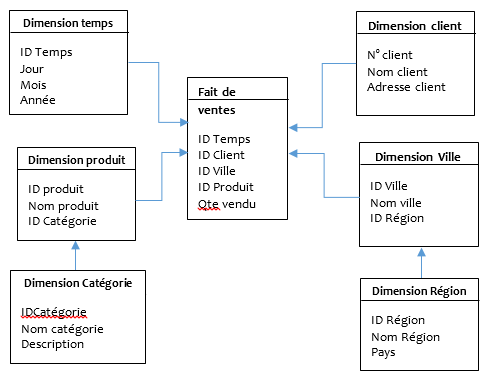
\includegraphics[width=\textwidth]{exempleflocon}
    \caption{Exemple de modèle en flocon}
    \label{fig:exempleflocon}
\end{figure}

\subsubsection{Modèle en constellation}
Ce n’est rien d’autre que plusieurs modèles en étoile liés entre eux par des dimensions communes. Comme dans la figure \ref{fig:exempleconstellation}
\begin{figure}[H]
    \centering
    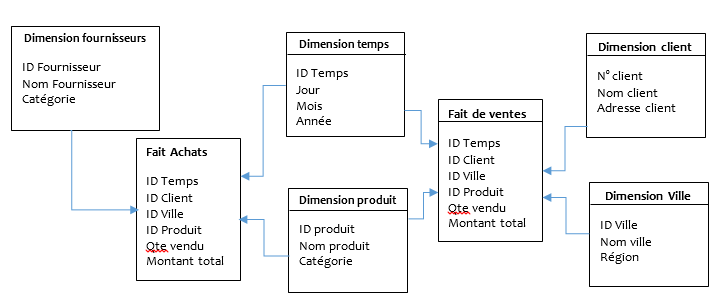
\includegraphics[width=\textwidth]{exempleconstellation}
    \caption{Exemple de modèle en constellation}
    \label{fig:exempleconstellation}
\end{figure}

Pour des raisons de performances nous avons choisi de travailler avec le \textbf{modèle en étoile}. Avec l'évolution de la technologie, l'espace mémoire n'est plus un grand soucis vu que nous travaillons principalement avec des données textuelles et numériques.

Ceci pourrait rapidement aboutir à un \textbf{modèle en constellation} si nous avons plus d'une table de fait par la suite.

\subsection{Approche de Conception}

Les approches de conception d'entrepôt de données sont un aspect très important de la construction d'un entrepôt de données. La sélection de la bonne conception d'entrepôt de données pourrait faire gagner beaucoup de temps et économiser du coût du projet. Il existe deux approches de conception d'entrepôt de données différentes normalement suivies lors de la conception d'une solution d'entrepôt de données et en fonction des exigences de votre projet, vous pouvez choisir celle qui convient à votre scénario particulier. 

\subsubsection{Top-down Design (L'approche descendante)}

Dans l'approche descendante, l'entrepôt de données (datawarehouse) est conçu en premier, puis le magasin de données (datamart) est construit au-dessus de l'entrepôt de données. La figure \ref{fig:topdown} illustre le fonctionnement de l'approche descendante.

\subsubsection{Bottom-Up Design (L'approche ascendante)}

Selon cette méthode, les datamarts sont d'abord créés pour fournir la capacité de reporting et d'analyse pour un processus métier spécifique, puis avec ces data marts, un entrepôt de données d'entreprise est créé. Les datamarts sont directement chargés avec les données des systèmes source, puis le processus ETL est utilisé pour charger dans l'entrepôt de données. Illustration dans la figure \ref{fig:bottomup}

\begin{figure}[H]
    \centering
    \begin{minipage}{.5\textwidth}
      \centering
      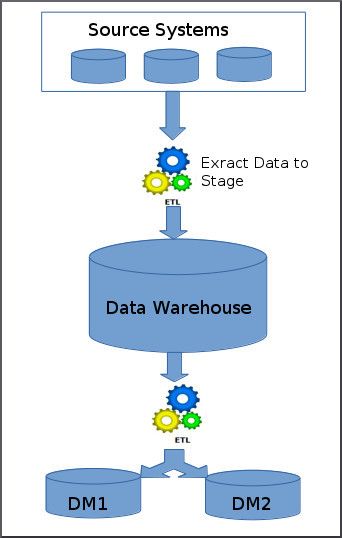
\includegraphics[width=.8\linewidth]{topdown}
      \captionof{figure}{Top-down Design}
      \label{fig:topdown}
    \end{minipage}%
    \begin{minipage}{.5\textwidth}
      \centering
      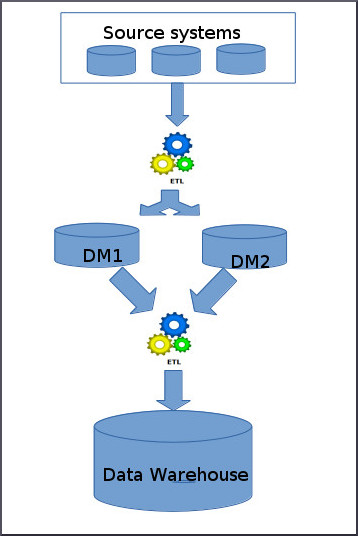
\includegraphics[width=.85\linewidth]{bottomup}
      \captionof{figure}{Bottom-Up Design}
      \label{fig:bottomup}
    \end{minipage}
\end{figure}


Pour notre projet nous utiliserons l'approche Top Down.




\subsection{Construction des tables de faits et de dimensions}
\subsubsection{Tables de fait}
Comme vu plus haut une table de fait est une table qui contient les données observables (les \textbf{faits}) que l'on possède sur un sujet et que l'on veut étudier, selon divers axes d'analyse (les dimensions).

Pour notre projet on a principalement deux(02) problèmes dont on fait face.
\paragraph{Comment fixer le prix d'un produit a une certaine periode}
On constate ici que la fixation des prix relève du sujet de ventes. Parce que la fixation des prix va améliorer les ventes. De là on peut déduire qu'on aura une table de fait <<Vente>> dans anotre datawarehouse. Pour connaitre ses attributs, il faut identifier les dimensions (axes d'analyse) pour ce fait.

Pour savoir comment fixer le prix d'un produit à une certaine période on a besoin d'analyser les ventes des produits. On doit ressortir les différentes axes d'analyse :
\begin{itemize}
    \item L'analyse par produit
    \item L'analyse par client
    \item L'analyse par temps
    \item L'analyse par ville
\end{itemize}
Ceux ci seront nos tables de dimensions et nous les construirons plus tard. Pour l'instant on utilisera juste leurs ID comme clé étrangère dans notre table de faits. Le reste des attributs seront les mésures pour chaque vente :
\begin{itemize}
    \item Quantité
    \item Prix Total
\end{itemize}

\paragraph{Comment éviter des commandes des produits indisponible :} Ici on sait que la solution c'est d'avoir en stock le produit excatement au moment de la demande (commande). On aura donc une table de fait de \textit{<<Commande>>}. Pour avoir cet information on doit analyses les dimensions suivantes :
\begin{itemize}
    \item Le produit
    \item Le temps
    \item Le client
\end{itemize}
Pour compléter ses attributs ressort les faits des commandes :
\begin{itemize}
    \item La quantité
    \item Valeur nette
    \item Disponibilité
\end{itemize}

Nous constatpns que nous auront 2 tables de fait, \textbf{Vente et Commande}.



\subsubsection{Tables de dimension}
Rappelons que une dimension est une table qui contient les axes d’analyse (les \textbf{dimensions}) selon lesquels on veut étudier des données observables (les faits) qui, soumises à une analyse multidimensionnelle, donnent aux utilisateurs des renseignements nécessaires à la prise de décision.
\paragraph{}
Des faits qu'on a identifié plus haut nous avons ressorti les dimensions qui seront présentes dans notre datawarehouse. On constate qu'il ya des dimensions qui sont présentes pour les deux fait alors on ne les implémente pas doublement.

\begin{itemize}
    \item Produit
    \item Temps
    \item Client
\end{itemize}


\subsection{Conception du schéma global du Datawarehouse}
La figure \ref{fig:schemaglobaldwh} représente le schéma de notre datawarehouse.

\begin{figure}[H]
    \centering
    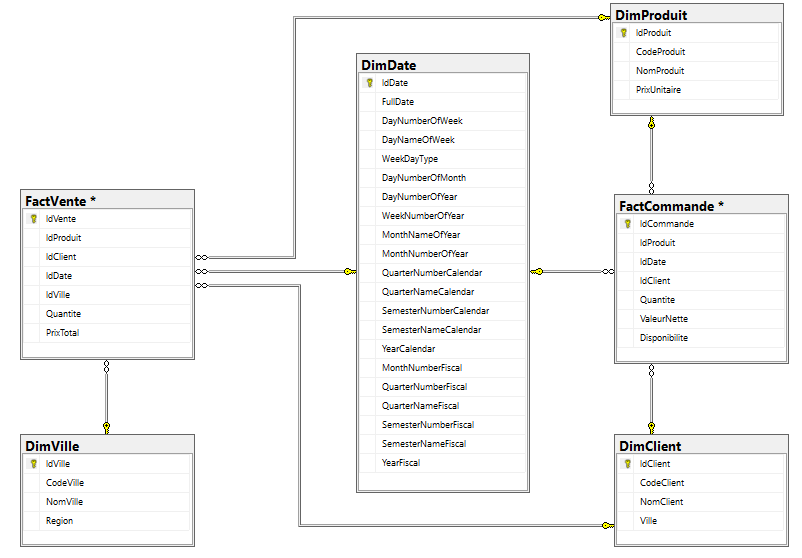
\includegraphics[width=\textwidth]{schemaglobaldwh}
    \caption{Schéma Global du Datawarehouse}
    \label{fig:schemaglobaldwh}
\end{figure}

\subsection{Construction des Datamarts}
A partir de notre datawarehouse, on constate qu'on a deux tables de faits. Ceux ci correspondent a deux datamarts qu'on peut analyser différement.

\subsubsection{Datamart de Vente}
La table de fait Vente et ses tables de dimension représentent les composant du datamart de Vente. Ce datamart aura pour objectif d'analyser les ventes pour en ressortir d'informations utiles pour la fixation des prix des produits.

La figure \ref{fig:datamartvente} représente le schéma du datamart de Vente.

\begin{figure}[H]
    \centering
    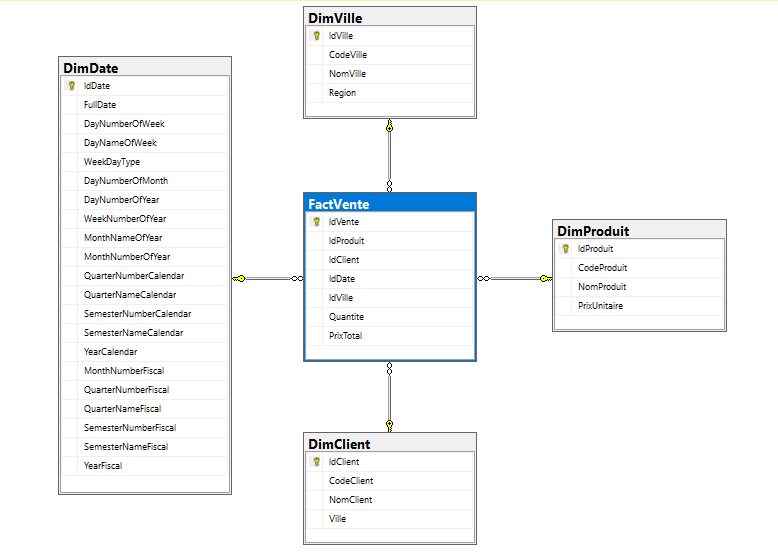
\includegraphics[width=\textwidth]{datamartvente}
    \caption{Datamart de Vente}
    \label{fig:datamartvente}
\end{figure}

\subsubsection{Datamart de Commande}
La table de fait Commande et ses tables de dimension représentent les composant du datamart de Commande. Ce datamart aura pour objectif d'analyser les commandes pour en ressortir d'informations utiles pour savoir a quel moment se ravitailler sur certains produits, évitant ainsi des clients insatisfaits.

La figure\ref{fig:datamartcommande} représente le schéma du datamart Commande.
 
\begin{figure}[H]
    \centering
    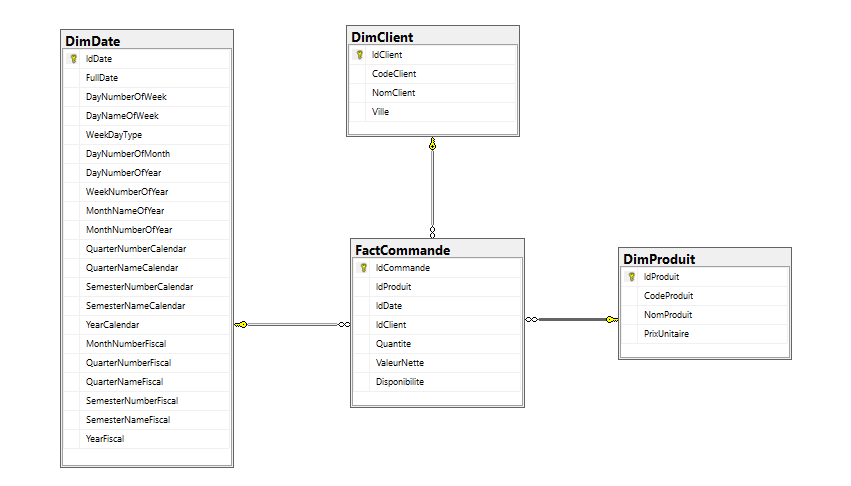
\includegraphics[width=\textwidth]{datamartcommande}
    \caption{Datamart de Commande}
    \label{fig:datamartcommande}
\end{figure}

\section{Conception des ETL}

\subsection{Architecture du processus ETL}
Un processus ETL du debut a la fin s'appelle generalemnt  un pipeline. La figure \ref{fig:etlarchitecture} extrait d'un site de formation en ligne Element61\footnote{https://www.element61.be/en/competence/best-practice-etl-architecture} decrit l'architesture des ETL qui seront mis sur peid pour l'alimentation de notre datawarehouse.

\begin{figure}[H]
    \centering
    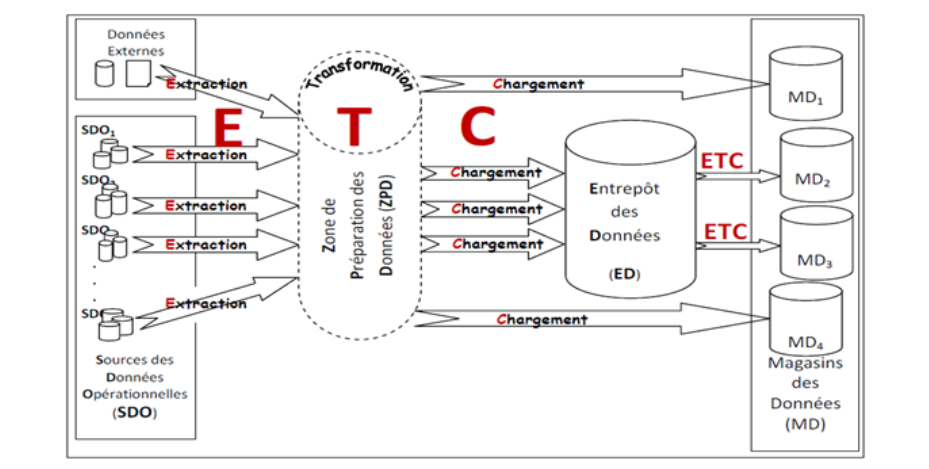
\includegraphics[width=\textwidth]{etlarchitecture}
    \caption{Architecture de l'ETL}
    \label{fig:etlarchitecture}
\end{figure}

%\subsection{Taches et étapes de l’ETL}


\subsection{Extraction des données}
Un processus ETL du début à la fin s'appelle généralement un pipeline ETL. L’extraction qui est la première phase du processus ETL consiste à définir les différents composants (tâches) qui seront connectes à nos sources de données. Ces composants iront lire les données et les achemineront dans le pipeline ou ils seront traités. Il existe plusieurs tâches permettant de lire les données dépendant du type de source de données. Dans notre cas nous avons nue base de données de production et aussi des fichiers plats. Alors nous allons définir deux types de taches à utiliser.
\begin{itemize}
    \item \textbf{Pour la base de donnes de production} on utilisera une connexion ODBC\footnote{Online DataBase Connectivity} qui nous permettra d’établir une connexion avec la base de données de production. On insèrera les paramètres de connexion et choisiront la table de laquelle nous voulons extraire les données. 
    \item \textbf{Pour les fichiers plats} nous utiliseront la connexion aux fichiers plats, ou nous préciseront simplement le chemin vers les fichiers qu’on souhaite lire. Ces données seront lues et achemines vers les tâches de traitement.
\end{itemize}

\subsection{Transformation des données}
La transformation c’est l’étape de l’ETL ou on fait des traitements nécessaires sur les donnes. Dans notre cas le seul traitement à faire qui est de s’assurer que les donnes provenant de la sources sont du même type que les tables dans lesquels ils von être chargés. 

\subsection{Chargement des données}
Puisque nous avons un seul type de destination pour tous nos données, qui est une base de données SQL, nous avons un seul type de connexion à implémenter, qui est la connexion OLEDB\footnote{Object Linking and Embedding, Database}. Nous allons préciser les paramètres de connexion à notre base de donnes de STAGING et nous connecter pour permettre aux données traitées d’être chargées dans la base de données.

\subsection{Alimentation du Datawarehouse}
La STAGING comme on le sais est une base de données temporaire de préparation de donnes. Bien que la DATAWAREHOUSE ne soit pas normalisée, la STAGING l’est encore mois. Les donnes dans la STAGING contiennent généralement les donnes tels qu’elles sont, ou presque dans les sources. De ce fait il nous faut les rendre un peu plus propre et conforme aux traitements par les cubes avant de les charger dans la DATAWAREHOUSE. Ceci se fera à travers une procédure stockée que nous créerons dans la base de données. Nous aurons donc une tache d’exécution SQL qui aura pour simple but d’exécuter notre procédure stockée créée.


\subsection{Alimentation des Datamarts}
Tout comme l'alimentation de la DATAWAREHOUSE, les datamarts seront alimentées par des procédures stockées. Ces procédures auront pour but d’aller sélectionner les données correspondantes à chaque datamart et les charger dans la datamart en question. On aura plus besoin de traitements puisque tout a déjà été fait avant de charger la DATAWAREHOUSE.

\subsection{Schémas des ETL conçus }
\subsubsection{ETL de chargement dans la STAGING}
Pour chaque table présente dans notre DATAWAREHOUSE une table correspondante est présente dans la STAGIING. Et chacune de ces tables (sauf la Dimension Date) doit avoir un ETL pour son chargement. Ces ETL auront tous le même schéma, juste différentes tables source. Le schéma de l’ETL est dans la figure \ref{fig:etlstaging}. 

\begin{figure}[H]
    \centering
    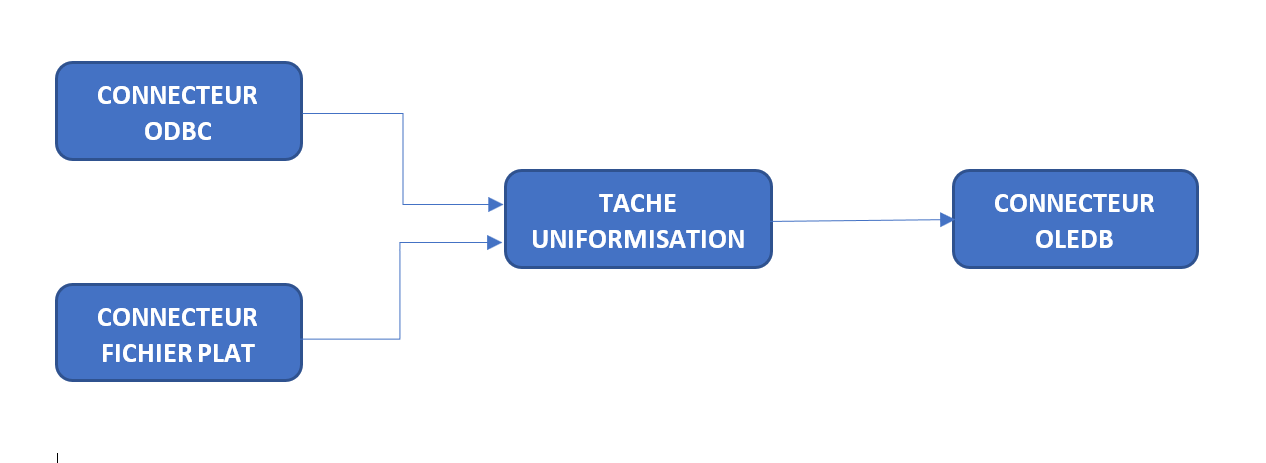
\includegraphics[width=\textwidth]{etlstaging}
    \caption{Architecture de l'ETL de chargement de la STAGING}
    \label{fig:etlstaging}
\end{figure}

\subsubsection{ETL d'alimentation de la DATAWAREHOUSE}
Puisque pour alimenter la DATAWAREHOUSE on a juste une procédure stockée à exécuter, l’ETL comportera juste une tache d’exécution SQL comme dans la figure \ref{fig:etldwh}

\begin{figure}[H]
    \centering
    
\includegraphics[width=\textwidth]{etldwh}
    \caption{Architecture de l'ETL de chargement de la DATAWAREHOUSE}
    \label{fig:etldwh}
\end{figure}

\subsubsection{ETL d'alimentation des Datamarts}
Comme pour la DATAWAREHOUSE, ici on a juste une procédure stockée à exécuter, et donc l’ETL comportera juste une tache d’exécution SQL comme dans la figure \ref{fig:etldwh}

% \section{Conception des cubes OLAP}


% \section{Conception du reporting (La visualisation) - La méthode UI/UX}


\section*{Conclusion}%
\addcontentsline{toc}{section}{\numberline{}Conclusion}%
Avec pour objectif de concevoir les différents composants pour mettre sur pied notre entrepôt de données dans ce chapitre, nos résultats nous permettent de passer à la partie réalisation de notre projet.


